\documentclass[a4paper, 11pt]{article}

\usepackage[spanish]{babel}
\usepackage[utf8]{inputenc}
\usepackage[vmargin=2cm,hmargin=2cm]{geometry}
\usepackage{enumerate}
\usepackage{dsfont}
\usepackage{graphicx}

\title{\Huge \textbf{Descripción del problema\\DDSI}}

\author{Antonio Checa Molina \\ Iñaki Madinabeitia \\ Bruno Santidrián \\ Darío Sierra}

\date{\today}


\begin{document}

\maketitle
\tableofcontents

\newpage
\section{Gestión de un registro de partidas en juegos generales}

El problema a resolver es mantener un registro rápido y funcional de partidas para cualquier tipo de juegos, deportes o competiciones con el fin de facilitar análisis y entrenamiento de jugadores. Hay que desarrollar un sistema de información de organización de las partidas y de los juegos.

Al principio, un grupo de gestores necesita proporcionar información de un juego y de sus partidas: aquello que se guarda, como la puntuación, los equipos, los jugadores de los equipos o un vídeo del partido. Una vez guardados estos atributos, el usuario podrá acceder al registro de partidas de un juego concreto e incluir aquellas de las que tenga datos. 

Por ejemplo, si se añade el juego baloncesto junto a un conjunto de atributos como \{Puntuación, Equipos, Puntuación de cada parcial, vídeos\}, cada partida contendrá esta información y los usuarios podrán acceder a esta. En esta práctica nos restringiremos a un pequeño número de juegos, realizando el diseño de base de datos para cada uno.

\subsection{Consulta}
\subsubsection{Esquema Entidad/Relación:}

\begin{figure}[h!]
	\centering
	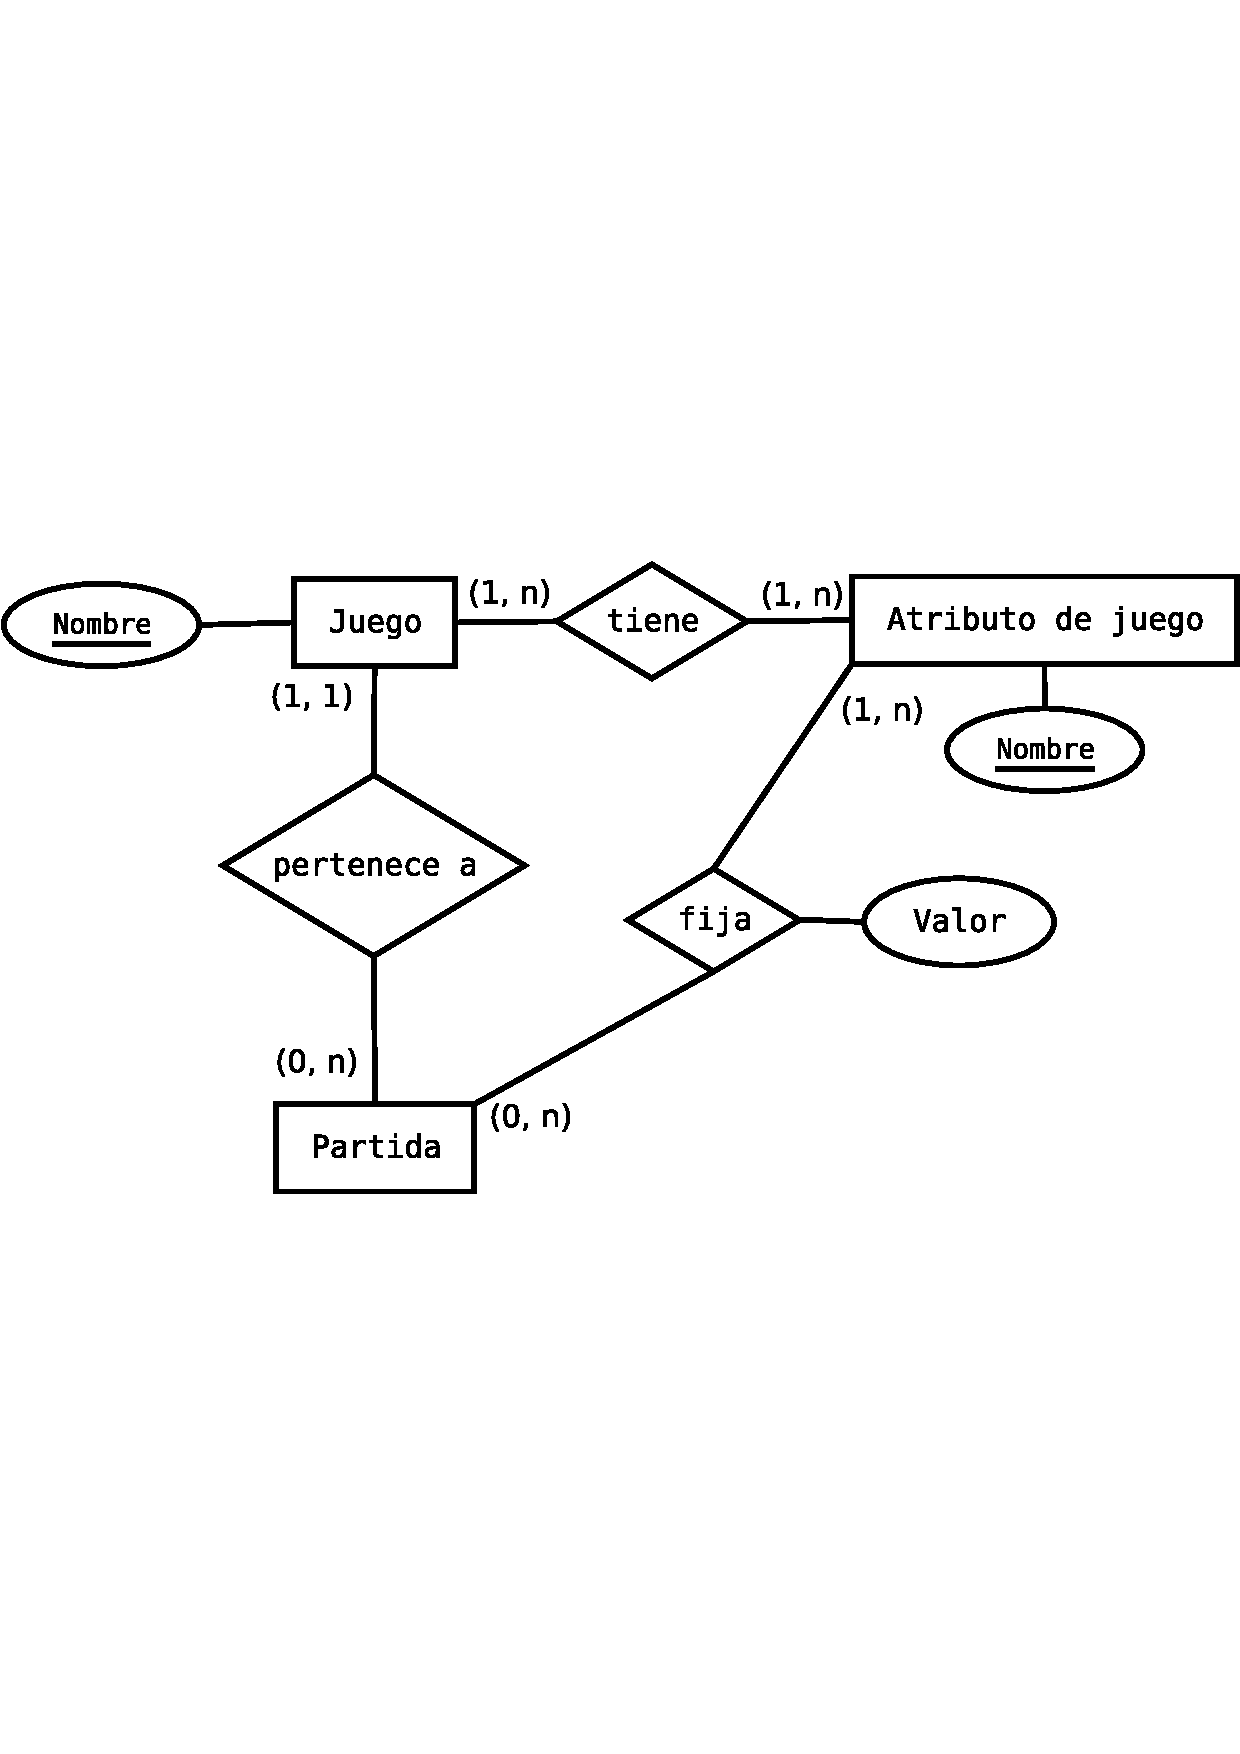
\includegraphics[width=0.7\linewidth]{../Diagramas/pdf/ER-Consulta.pdf}
	\caption{Diagrama ER del subsistema Consulta.}
	
	\label{fig:ERConsulta}
\end{figure}

\subsubsection{Diagramas de flujo de datos:}

Refinamos el proceso Consulta en sus cuatro requisitos funcionales  y realizando la descomposición del almacén en Partidas y Atributos mediante una primitiva descendente de descomposición en procesos sin conexiones.
 
\begin{figure}[h!]
\centering
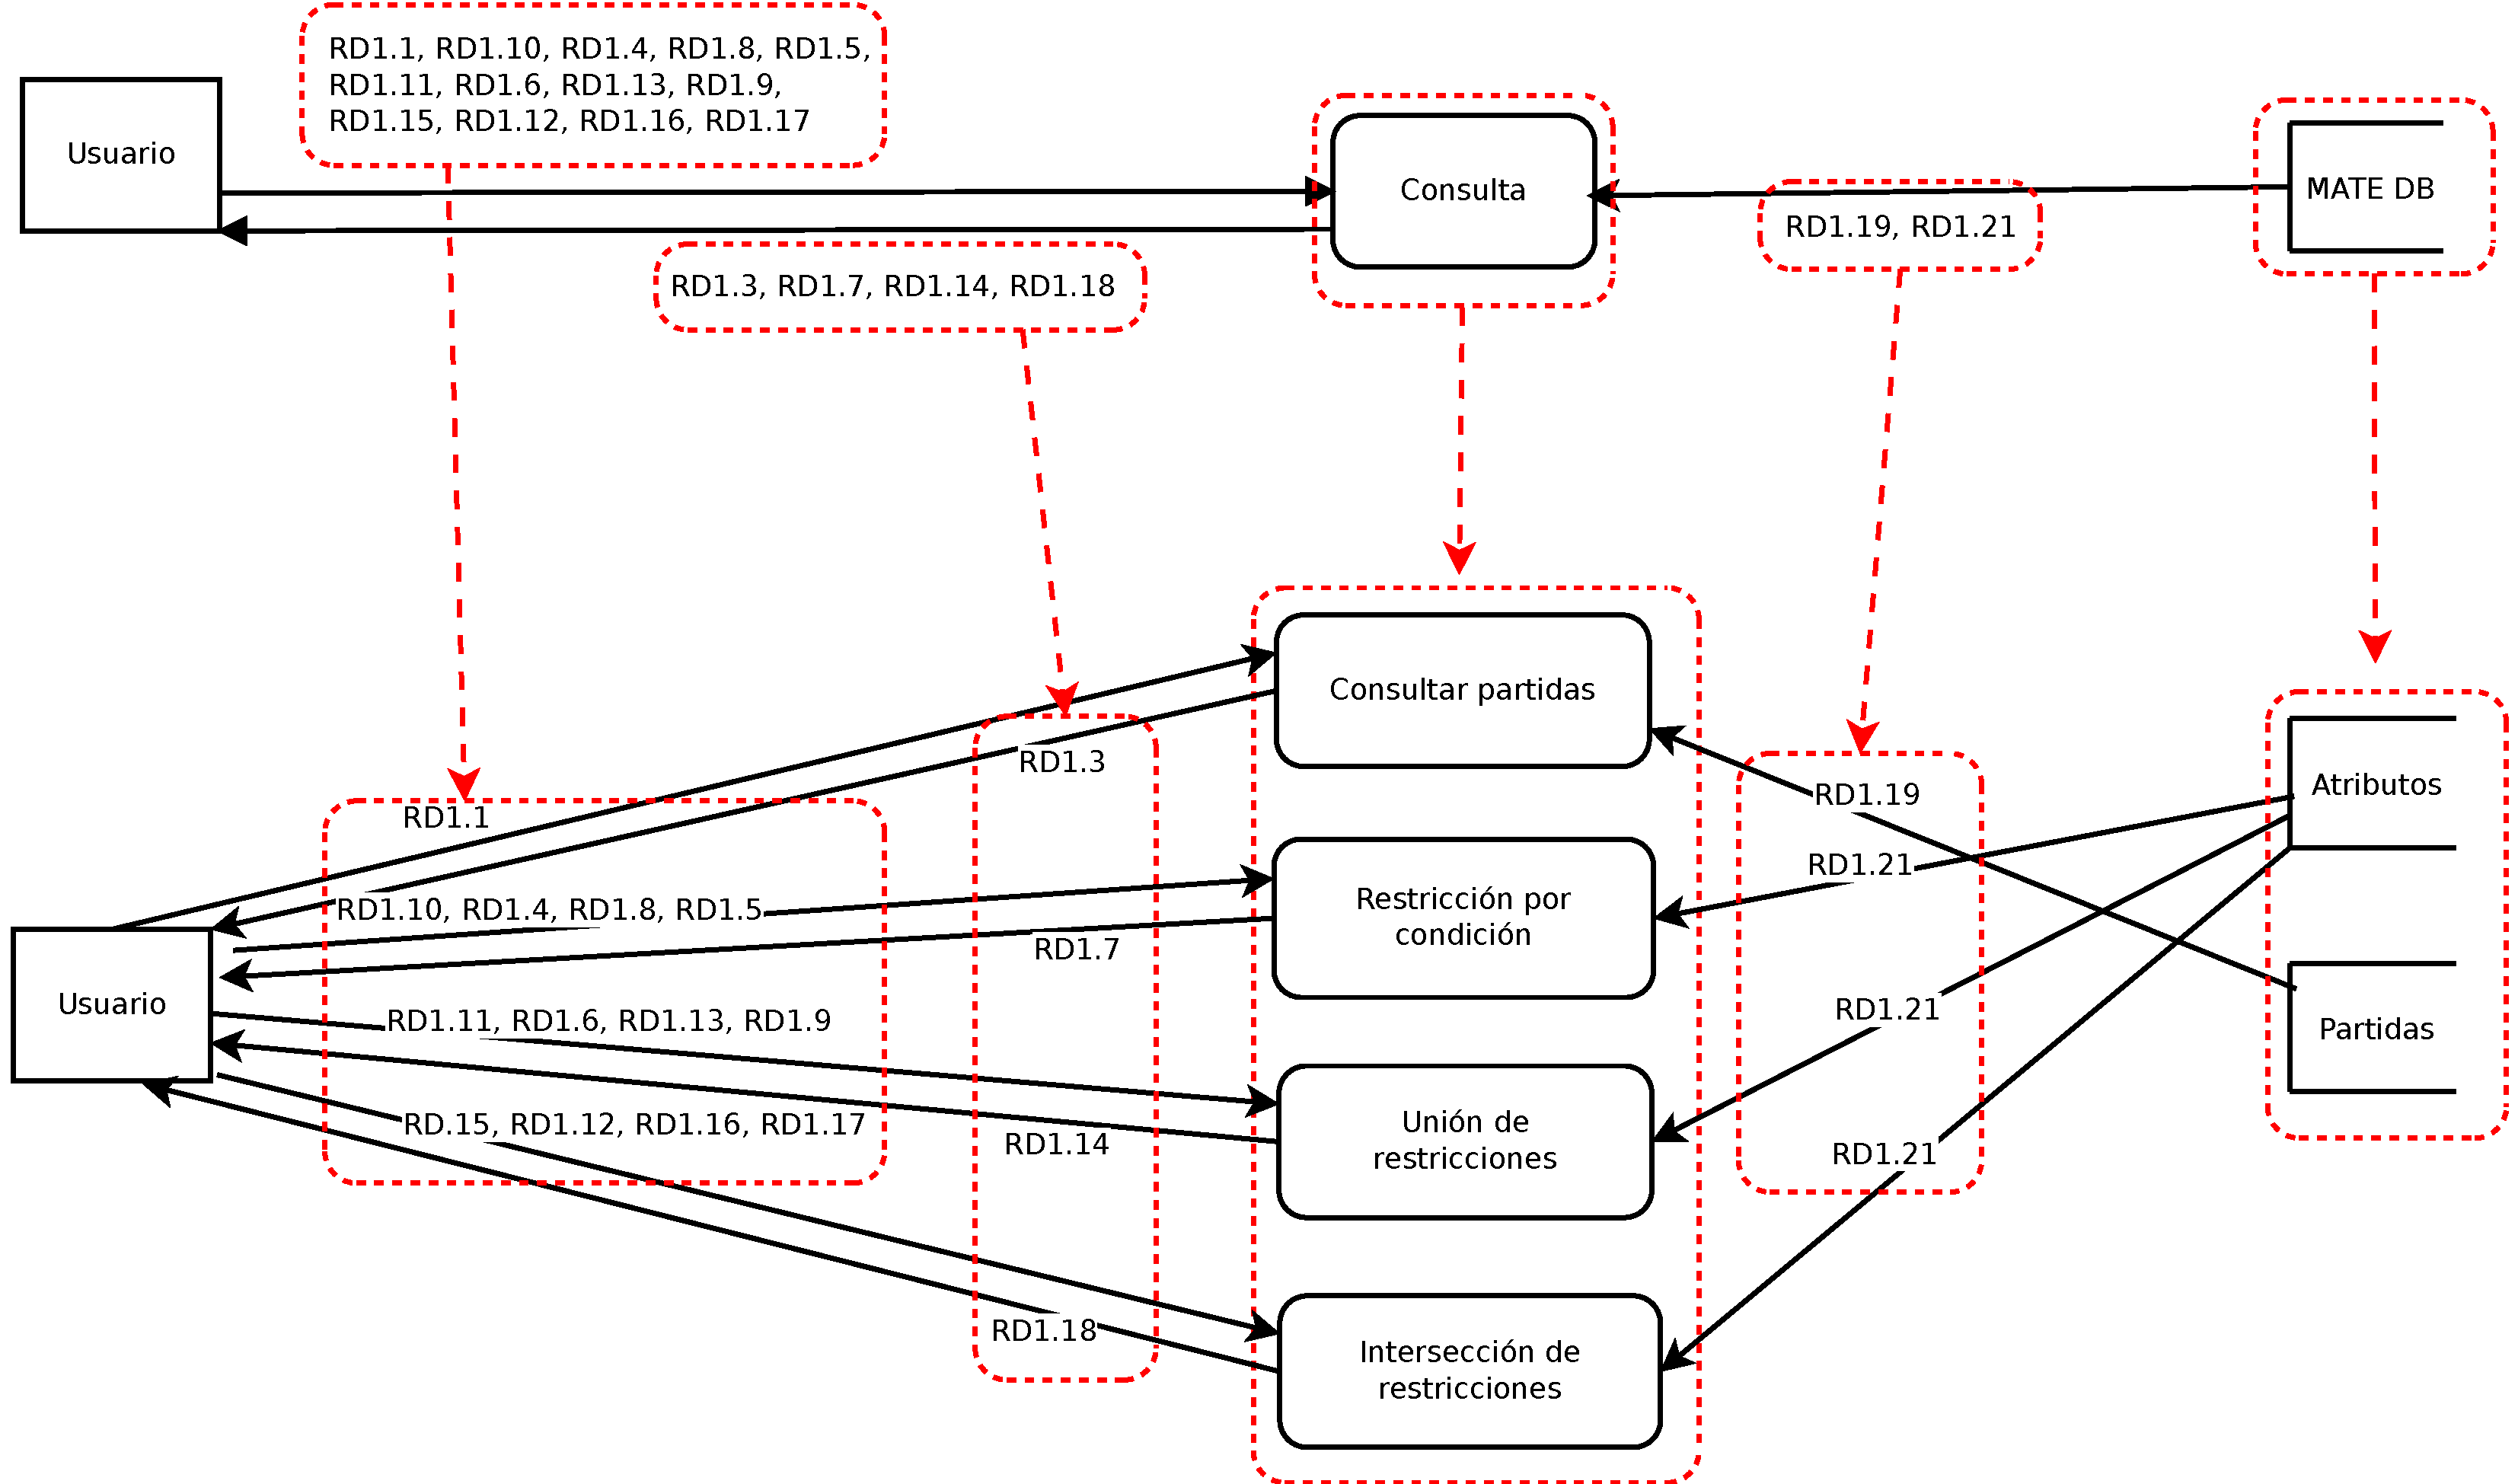
\includegraphics[width=0.7\linewidth]{../Diagramas/pdf/RefinamientoConsulta.pdf}
\caption{Flujo de datos del subsistema Consulta.}

\label{fig:RefinamientoConsulta}
\end{figure}

\subsubsection{Esquema Externo:}

\begin{figure}[h!]
	\centering
	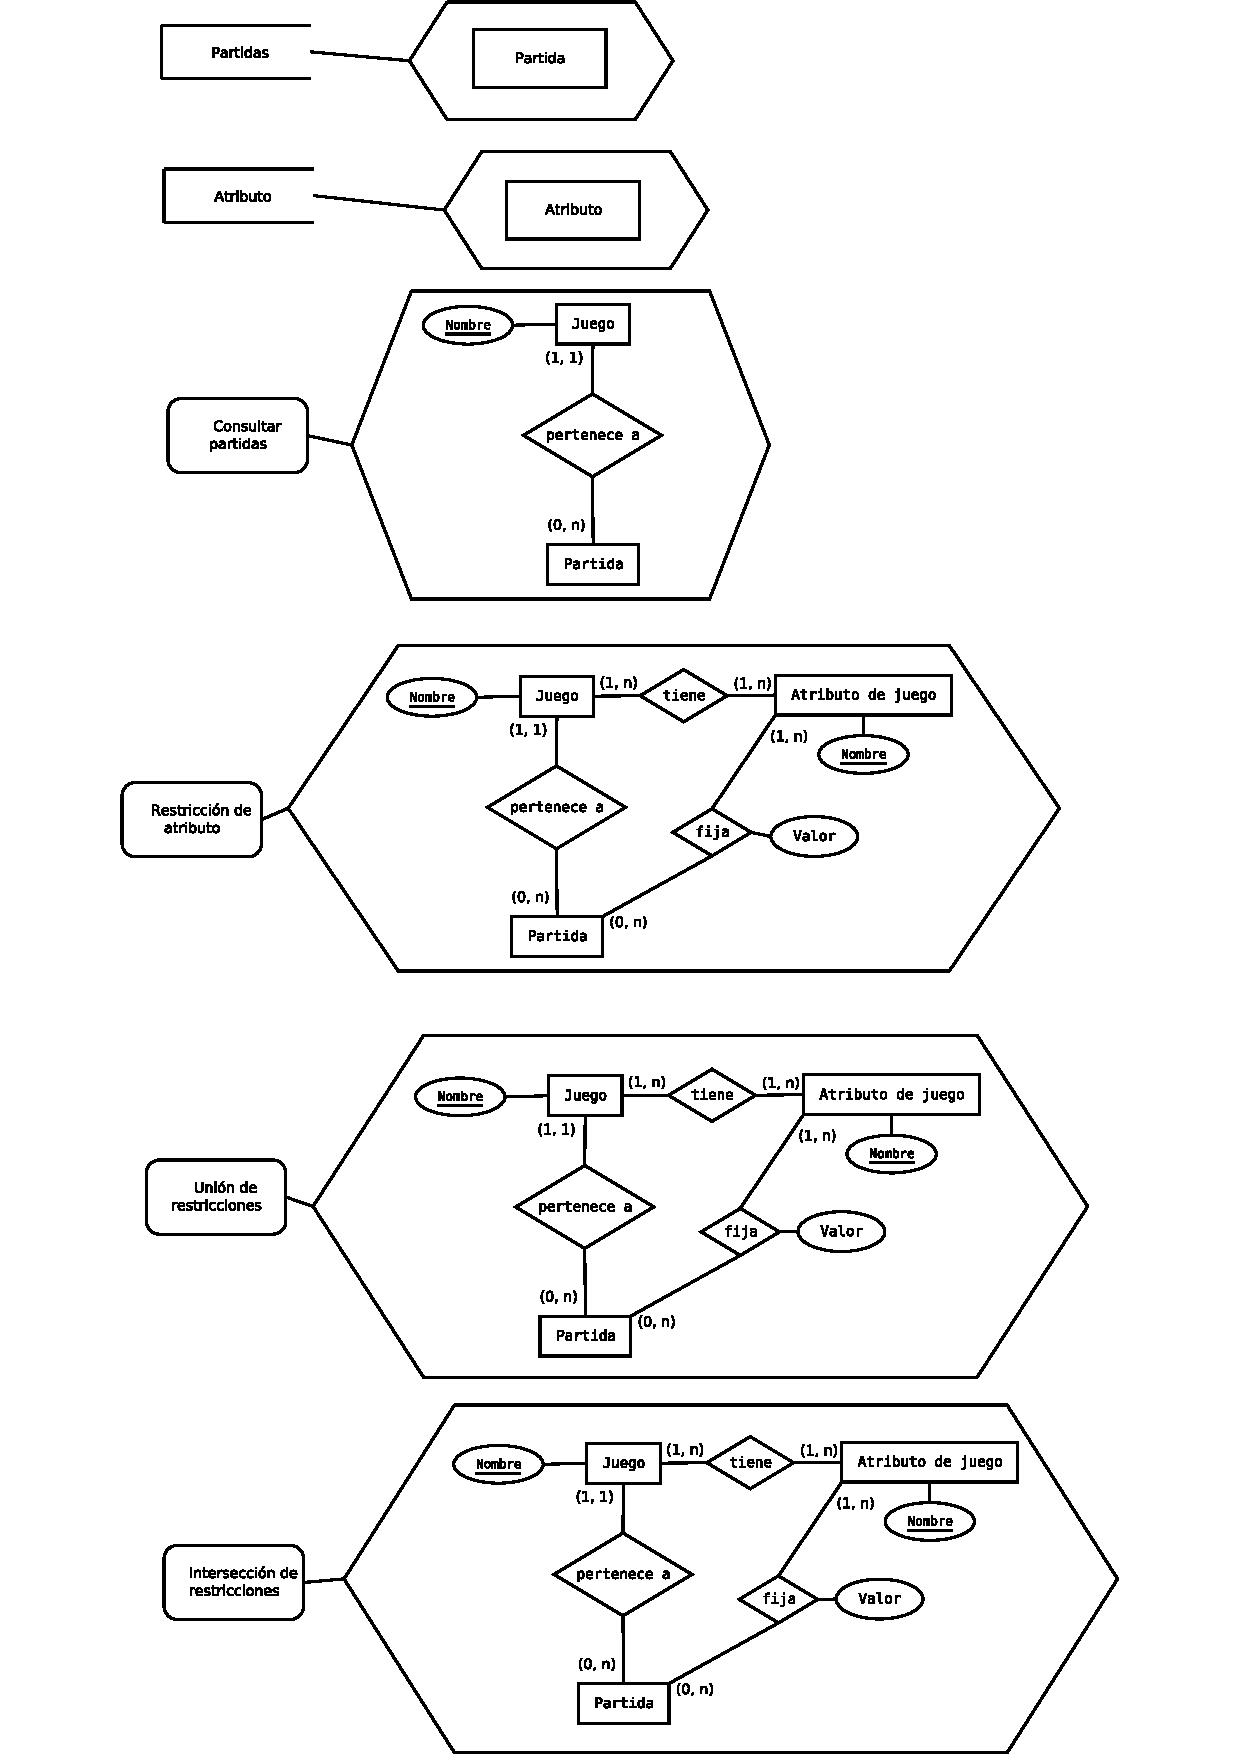
\includegraphics[width=0.7\linewidth]{../Diagramas/pdf/EsquemaExternoConsulta.pdf}
	\caption{Esquema externo de Consulta.}
	
	\label{fig:EsquemaExtConsulta}
\end{figure}


\subsection{Consejos}
En todos los juegos en los que se guarde el estilo de juego, la aplicación
aconseja cómo jugar en determinadas condiciones, recomendando al usuario aquellos
estilos que más probabilidades tengan de ganar.\\

Dado un juego, el usuario podrá elegir uno o varios atributos de este (e.g. estilo
de juego en un partido de baloncesto: ofensivo o defensivo) y ciertos datos extra,
como el oponente al que se quiere enfrentar, o ciertos valores de los atributos 
que puede tener el oponente y el sistema analiza los datos guardados en la base
de datos para aconsejar unos valores que puedan ser beneficiosos (e.g. jugar ofensivo).\\

El subsistema debería dar información extra sobre el proceso de como ha elgido los
valores de los atributos, como el número de jugadas analizadas y la fiabilidad de los datos.\\

También es posible que el subsistema de consejos use funcionalidades del subsistema
de estadísticas, siempre que dicha funcionalidad esté implementada, para que las
recomendaciones sean más certeras.\\



\subsection{Inclusión de partidas}
La inclusión de las partidas necesita que el usuario incluya aquellos atributos vitales en una partida, pudiendo o no incluir los opcionales. Necesitaría insertarlos por la interfaz gráfica.\\

El sistema de información que planteamos crear deberá incrementar el número de juegos disponibles con el avance del tiempo, para asegurar su uso continuado. Por tanto, distinguimos entre inclusión de juegos (trabajo de los administradores de la base de datos) y la inclusión de partidas (trabajo de los usuarios).\\

Una partida será un registro más de la tabla de datos asociada a cada juego. Como atributo vital se necesitará añadir el nombre del juego, así como la puntuación final de dicha partida; estos serán atributos comunes a cada a todas las partidas, pues todas pertenecerán a un juego y todas tendrán una puntuación asociada.\\

Los atributos opcionales serán aquellos inherentes a cada juego; no tiene sentido la inclusión de un atributo 'Jugadores del equipo' en un juego de cartas, ni un 'baraja del oponente' en uno que no lo sea. Aquí opcional no se entiende como 'poco relevante' pues estos atributos son la razón de ser del propio sistema de información. Los datos inherentes a cada juego, los que lo hacen distinguible del resto, serán objeto del análisis en el sistema.\\

Las partidas se incluirán desde la interfaz gráfica, donde una vez seleccionado el tipo de juego, se abrirán una serie de atributos (a definir por los administradores del sistema) que permitirán al jugador guardar su partida. Entre estos podremos encontrar: 'Jugadores del equipo', 'Mi Baraja', 'Baraja del oponente', 'Número de faltas cometido', 'Pichichi del encuentro', etc.\\

Aunque hemos clarificado que la inclusión de partidas debe ser trabajo de los usuarios, en juegos específicos (fútbol, baloncesto, etc), en los que, a diferencia de una partida entre dos jugadores de ajedrez, no queda claro quién debe almacenar el resultado. Es por esto, que se estudiará la posibilidad de responsabilizar a los administradores de mantener la base de datos actualizada para los juegos en los que se de esta situación.


\subsection{Estadísticas}
Por último, el sistema debería agregar las estadísticas que pida el usuario. Hay diversos modos de generar una gráfica. El usuario tendrá que indicar al sistema qué modo de salida de los datos quiere (por ejemplo, una gráfica 2D con líneas). Una vez indicado, tendrá que añadir sobre qué atributos del juego quiere la gráfica de datos (por ejemplo, sobre la puntuación de los partidos de los Lakers en cada mes). Después, el sistema debe generar la representación elegida de los datos en caso de que pueda y presentarla ante el usuario. En caso de que no pueda deberá mostrar un mensaje de error mencionando la causa.

Los posibles modos de una gráfica son: gráfico 2D (al menos el eje Y debe ser numérico), gráfico 3D (al menos el eje Y debe ser numérico), columna agrupada (al menos dos elementos numéricos por cada uno no numérico), circular (atributos numéricos positivos).

Al tratar los atributos el usuario debe ser capaz de realizar funciones como la media, la suma o contar datos que cumplan una restricción concreta. Para esto, el sistema debe ser capaz de proporcionar ayuda con todas las funciones que se pueden insertar, y gestionarlas para que funcionen como es debido.


Las estadísticas, datos y gráficas generadas se tendrán que guardar en el sistema, para que el usuario pueda acceder a ellas sin tener que generarlas de nuevo. Habrá acceso a un registro con orden inverso a la fecha de creación para facilitar la búsqueda en el mismo.

Cada modo de salida tiene unas restricciones sobre los atributos, en el caso en el que el usuario incluya unos datos erróneos para una gráfica concreta (por ejemplo, seleccionar el modo de disco para representar datos que no son números). En este caso, el error tendrá que hacer referencia al error concreto, y mostrarlo por pantalla para que el usuario entienda qué ha pasado. 

	
\end{document}
